The deterministic model, illustrated in system \ref{eq:System1} and implemented by the authors using the standard ode45 function in Matlab, resulted in the production of Figure \ref{fig:det_fitting}.
\begin{figure}[ht]
  \centering
  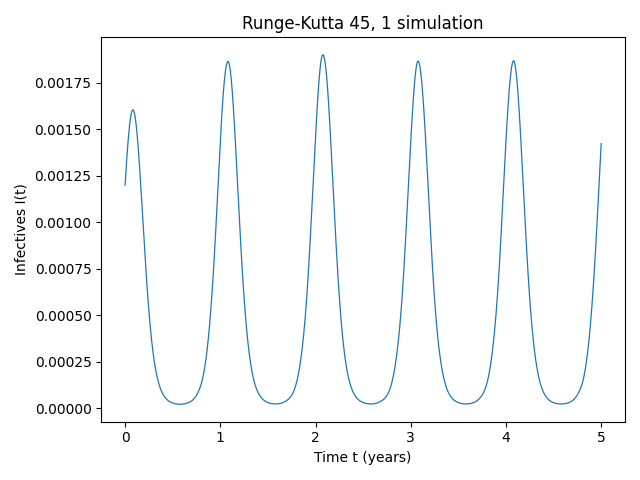
\includegraphics[width=0.8\textwidth]{IMG/2Det_solve_ivp_I(t).png}
  \caption{Adaptive step size Runge Kutta simulation obtained from the function \textit{solve\_ivp} of the python library scipy}
  \label{solve_ivp}
\end{figure}
 On our end, as said before, we employed the use of \textit{solve\_ivp}, from Scipy\cite{2020SciPy-NMeth} with default parameters, in python and obtained a comparable result as shown in Figure \ref{solve_ivp}. Due to the deterministic nature of the simulation we didn't perform multiple runs.
